 \ifx\wholebook\relax\else
\input{../Common.tex}
\input{../macroes.tex}
\begin{document}
\fi

\chapter{Mazes, Spirals and Other Figures}\label{ch:xploopvar}

\begin{chapterfigure}
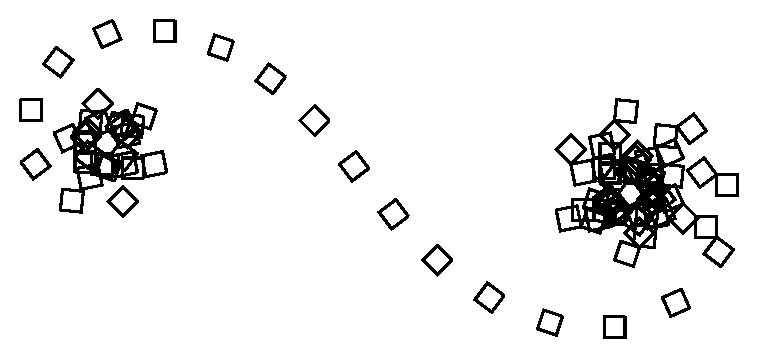
\includegraphics[width=9cm]{varLoopsfixedLengthSpiralfirstwithSquare}
\end{chapterfigure}

In Chapter~\ref{ch:loopvar} we propose you some experiments with loops and variables. At that time you were not aware that you could use other methods. Now we suggest you to redo these experiments but using other methods such as \ct{square:} and to define methods with multiple arguments to help you. As we already mentioned it, knowing how to solve complex problems using simpler methods is a difficult task that can only be learned by experience. Therefore we strongly suggest you to do all the following exercises and to try to find multiple solutions for each of them. 

\begin{exofigwithsizeandtitle}[0.5]{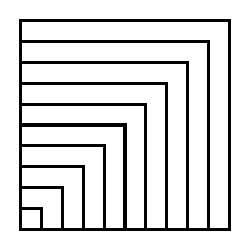
\includegraphics[width=6cm]{Argmirescr}}{Russian squares}\label{exo:russianSquares2}
Use the method \ct{square:} to build squares of different sizes as shown on the right figure.
\end{exofigwithsizeandtitle}

\begin{exofigwithsizeandtitle}[0.5]{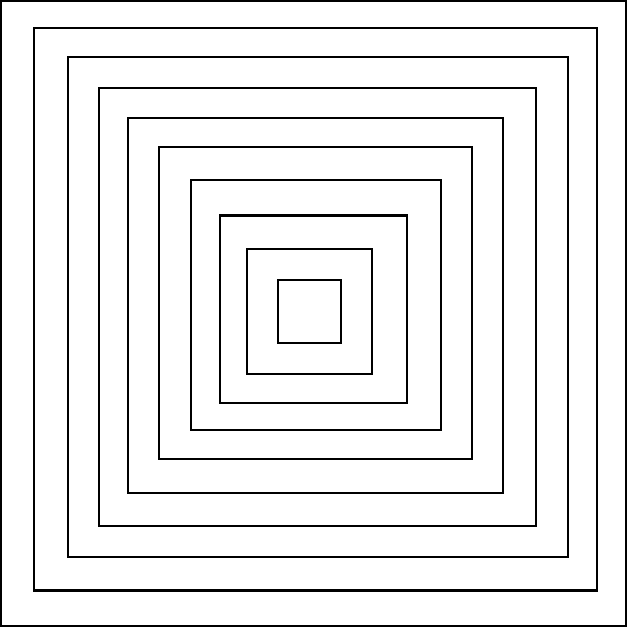
\includegraphics[width=6cm]{corridor}}{Corridor}\label{exo:corridorsimple2}
Build the squares of different sizes as shown on figure on the right.
\end{exofigwithsizeandtitle}



\begin{exofigwithsizeandtitle}[0.35]{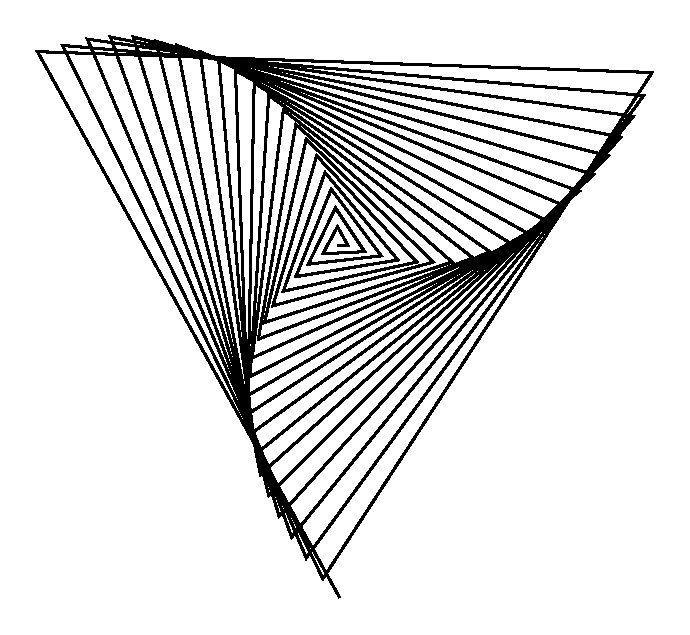
\includegraphics[width=8cm]{varLoopsSpiral121}}{Spiral}\label{exo:spiral}
Define the method \ct{spiral:} that given an angle draws a
spiral. Have fun and try different angle values, you can create
wonderful drawings.  The following script created the spiral shown on the right.
\begin{nalltt}
| \caro |
\caro := \Turtle new.
\caro spiral: 121
\end{nalltt}
\end{exofigwithsizeandtitle}

\begin{exonofig}
In the previous experiment,  you added each step a given number to the distance that the robot should move. Now experiment by computing the length of a side, not by adding a distance to the previous side length, but by multiplying by a given number. Pay
attention multiplying by 1.1 means an increase of 10\%.
\end{exonofig}

\begin{exonofig}
If we analyze a bit the way a spiral is drawn, we see that it depends on different 4 parameters, namely the \emph{number of sides}, the \emph{starting size} of a side, the \emph{amount the side is incremented} and the \emph{angle} to turn. Define a method named \ct{spiralNumber:size:add:angle:} that draws any spiral. Try for example the following scripts

\begin{nalltt}
| \caro | 
\caro := \Turtle new.
\caro spiralNumber: 50 size: 10 add: 3 angle: 144.
\caro color: Color red.
\caro spiralNumber: 120 size: 1 add: 3 angle: 12
\end{nalltt}
\end{exonofig}

\begin{exofigwithsize}[0.5]{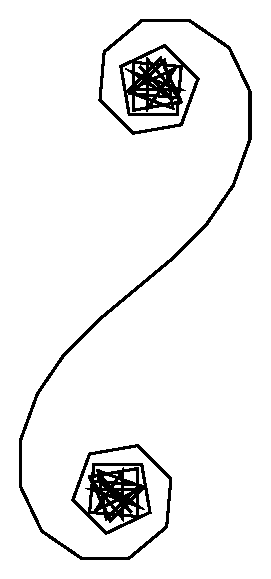
\includegraphics[width=3cm]{varLoopsfixedLengthOne}}\label{exo:crazy}
Up until now, we created spirals by \strong{changing the distance} of which the turtle moved forward and kept \strong{turning with the same angle}. Experiment by doing the opposite, keep the distance fixed but changed the angle with a fixed increment.
For that define a method with four arguments: the number of times you loop, the initial value of the angle, the angle increment and the length of a side.

As shown by Figure~\ref{fig:crazy}, trying to predict the curves generated by this method is quite difficult.  But fell free to play with different values. Have fun with it!  figure shown on the right is produced with 100 iterations, an initial angle of 40 degree, an increment of 5 and a size length of 23 pixels. Figure~\ref{fig:crazy} presents two other variations.
\end{exofigwithsize}



\begin{figure}[!htbp]
\begin{minipage}[c]{.5\linewidth}
\centerline{
\includegraphics[width=5cm]{varLoopsfixedLengthSpiral23}}
\end{minipage}
\begin{minipage}[c]{.5\linewidth}
\centerline{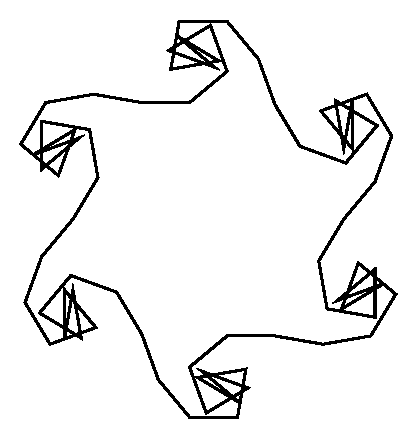
\includegraphics[width=5cm]{varLoopsfixedLengthSpiral72}}
\end{minipage}
\caption{Left: iterations: 90, initial angle: 2, increment: 20, length: 30. 
Right: iterations: 72, initial angle: 40, increment: of 30, length: 30.}
\label{fig:crazy}
\end{figure}


\begin{exonofig}%{varLoopsfixedLengthSpiralfirstwithSquare}
If you change the method that you defined in the \exoref{exo:crazy} and draw 
a small square instead of drawing a line, you can obtain really crazy pictures as the first one shown in this chapter.\end{exonofig}

\begin{exofig}{varLoopsHerisson}
Try to reproduce figure shown on the right. Here are some hints: start with a length of 5 and increase it 3 by 3, and turn an angle of 178 degrees.
\hidden{
\begin{nalltt}
| \caro length angle |
\caro := \Turtle new.
	length := 5.
	angle := 178.
	110 timesRepeat: [ caro go: length.
                 caro turnLeft: angle.
                 length := length + 3]
\end{nalltt}}
\end{exofig}








\ifx\wholebook\relax\else
\end{document}\fi
